\section{Influence Propagation}
\label{sec:influ}

As we discussed in Section~\ref{sec:meth}, 
many files are submitted to VirusTotal more than once, 
and more than 99\% submissions are analyzed by at least 50 anti-virus engines. 
We observe that some engines fail to identify some malwares during early submissions, 
but they catch up when analyzing later submissions. 
Anti-virus vendors frequently use VirusTotal to identify false negatives in their products, 
which are malwares they fail to detect but detected by other vendors. 
We assume that there are influence among different anti-virus vendors.
In this section, we try to model this influence,
and try to predict whether an engine will identify a file as malware in the future, 
after the engine has already labeled the file as benign.

\subsection{Influence Model}
\label{sec:model}

Influence propagation on social graph is a well-studied topic in web mining area. 
The static models we apply are proposed by~\citet{Influence} to analyze Flickr data.
In this section, we will first overview the static models~\cite{Influence} in our usage scenario, 
and then we will discuss how we use map-reduce to train models and use trained models to do prediction.  

We assume that all vendors form a complete directed social graph $G = (V, E)$, 
where the nodes $V$ are vendors. 
The social graph is complete, 
since we assume there is possible influence from any vendor to all other vendors.
We assume there are action logs generated, 
when VirusTotal applies a set of anti-virus engines to analyze a submission. 
For each engine, there will be an action log $(u, a, t)$ or an action log $(u, \bar{a}, t)$, 
representing whether or not $u$ takes action to identify the submission as a malware at time $t$. 
To make things easy, after a vendor $u$ labels a file as malware, 
we assume $u$ will insist its decision, 
and ignore cases where a vendor labels a file as malware, but labels the file as benign later. 

We use $A_u$ to represent the number of actions taking by u, 
or the number of malwares identified by $u$. 
We use $\bar{A}_u$ to represent the number of malwares ever analyzed and labeled as benign by $u$.
We use $A_{u\&v}$ to represent the number of actions taken by both $u$ and $v$, 
and $A_{u|v}$ to represent the number of actions taken by either $u$ or $v$.
Clearly, $A_{u|v} =   A_u + A_v - A_{u\&v}$
We use $A_{u2v}$ to represent the number of actions propagated from $u$ to $v$. 
We define action propagation as follows: 

\begin{definition}{Action Propagation:}
We say that an action $a$ propagated from $u$ to $v$ iff: (i) $\exists$ $(v, \bar{a}, t_i)$ $\in$ $\bar{A}_v$, 
and $(v, a, t_k)$ $\in$ $A_v$, with $t_i < t_k$; (ii) $\exists$ $(u, a, t_j)$ $\in$ $A_u$, with $t_j < t_k$. 
\end{definition}

For each edge $(u, v) \in E$ in the social graph $G$, 
there is an influence probability: $p_{u,v}$,
which represent after $u$ takes an action the probability that $v$ will follow $u$ to take the same action. 
Since social graph $G$ is a complete graph, 
all other nodes are all $v$'s neighbors. 
Let us use $S$ to represent the set of $v$'s neighbors, which take an action. 
The probability that $v$ will follow its neighbors to take the same action is

$$p_v(S) = 1 - \prod\limits_{u \in S}(1 - p_{u,v})$$

During training stage, we try to learn $p_{u,v}$ for each edge. 
During prediction stage, we provide a tunable threshold $\theta$. 
For node $v$ without taking an action, 
if $P_v(S)>\theta$, 
we predict $v$ will follow its neighbors to take the action in the future. 



\subsection{Experimental Results}

\begin{figure*}
\centering
\subfloat[]{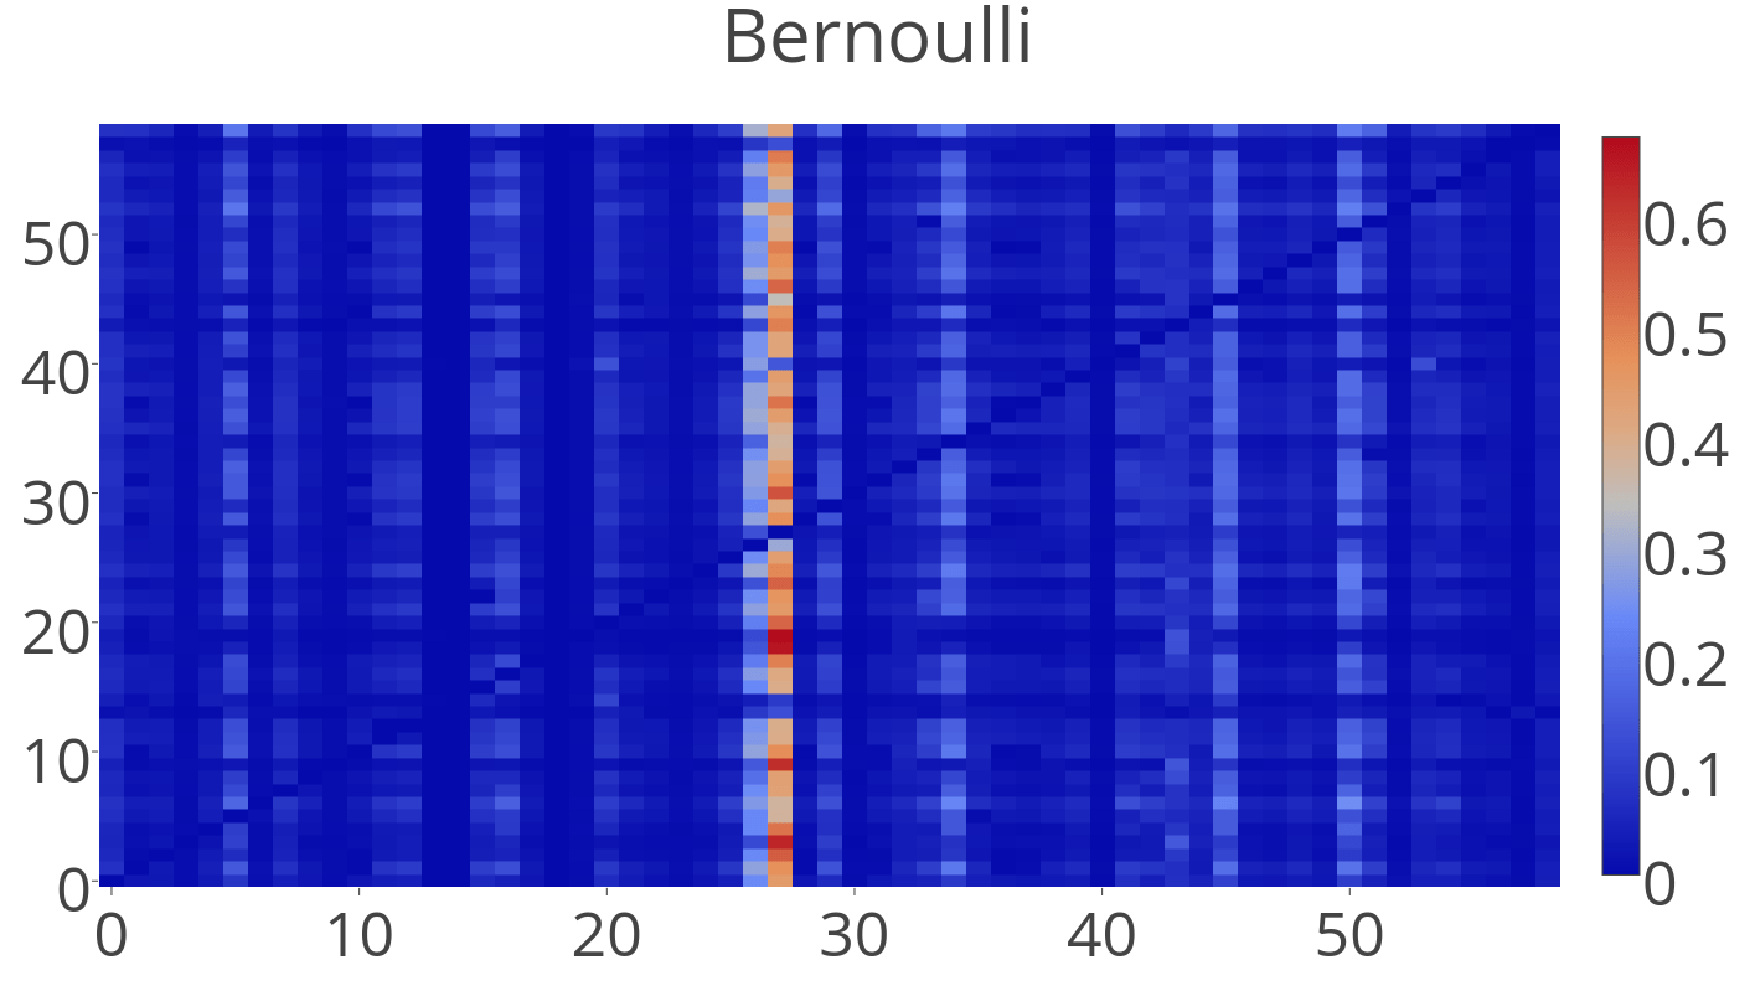
\includegraphics[width=0.24\linewidth]{figure/bernoulli-train}\label{fig:moredata1}} 
\subfloat[]{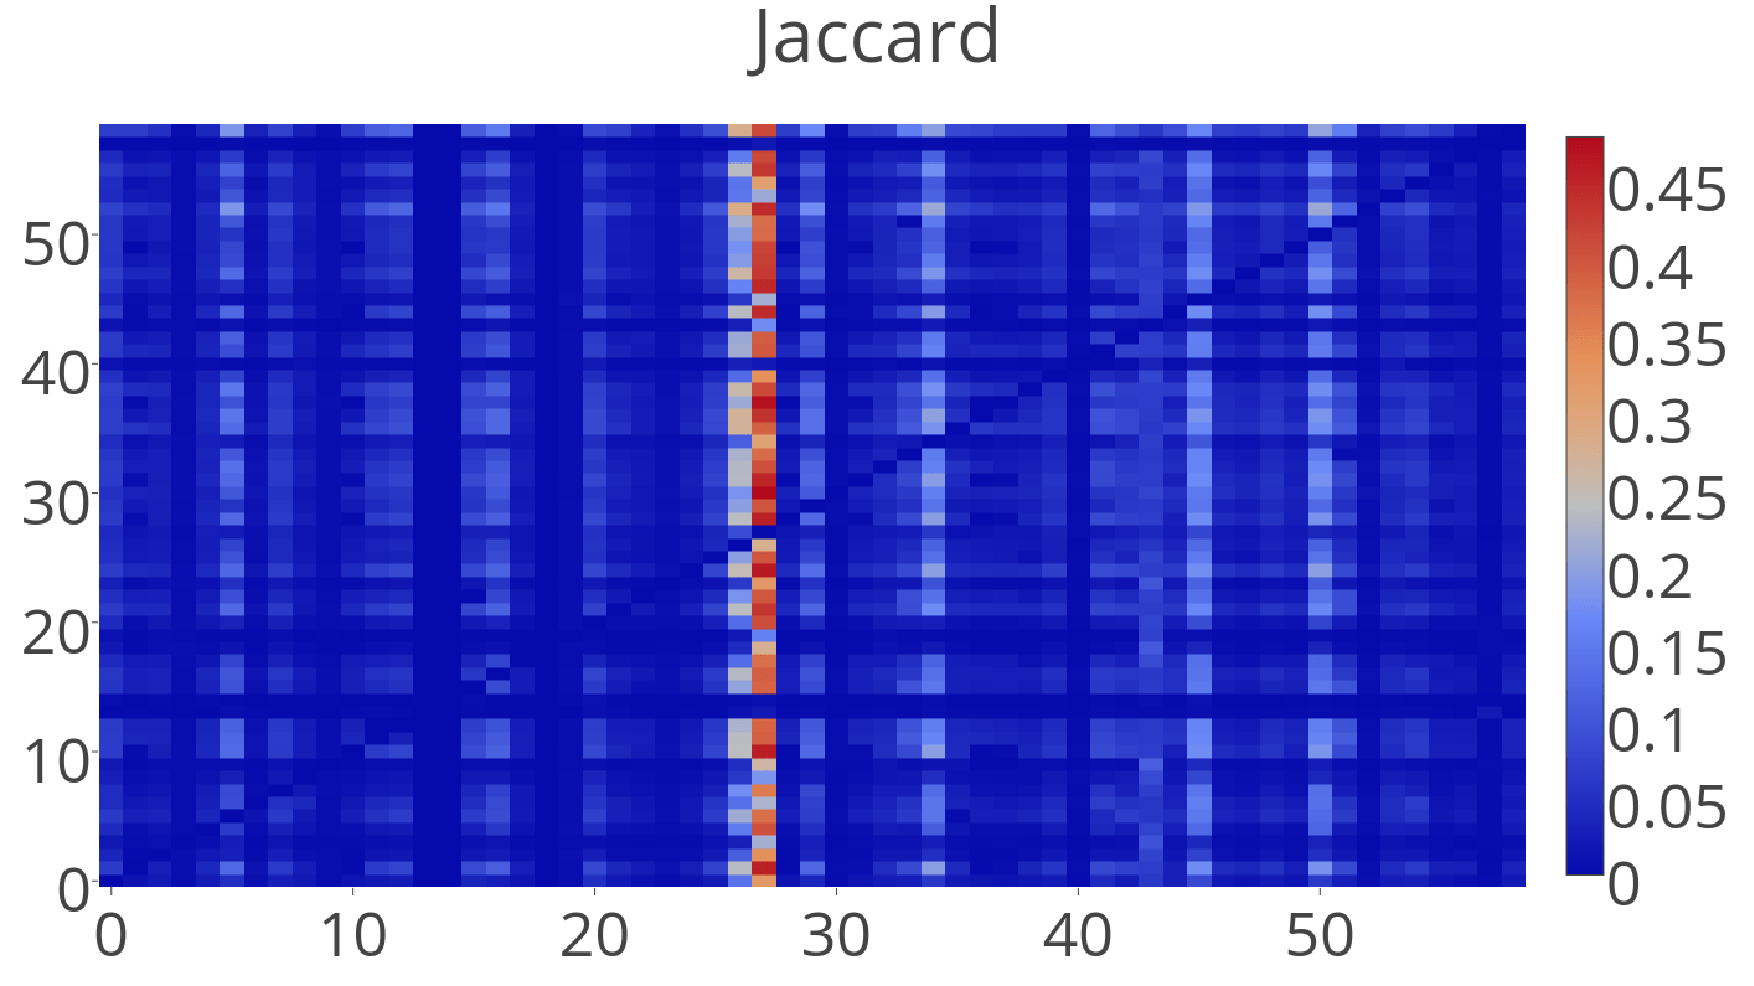
\includegraphics[width=0.24\linewidth]{figure/jaccard-train}\label{fig:moredata2}}
\subfloat[]{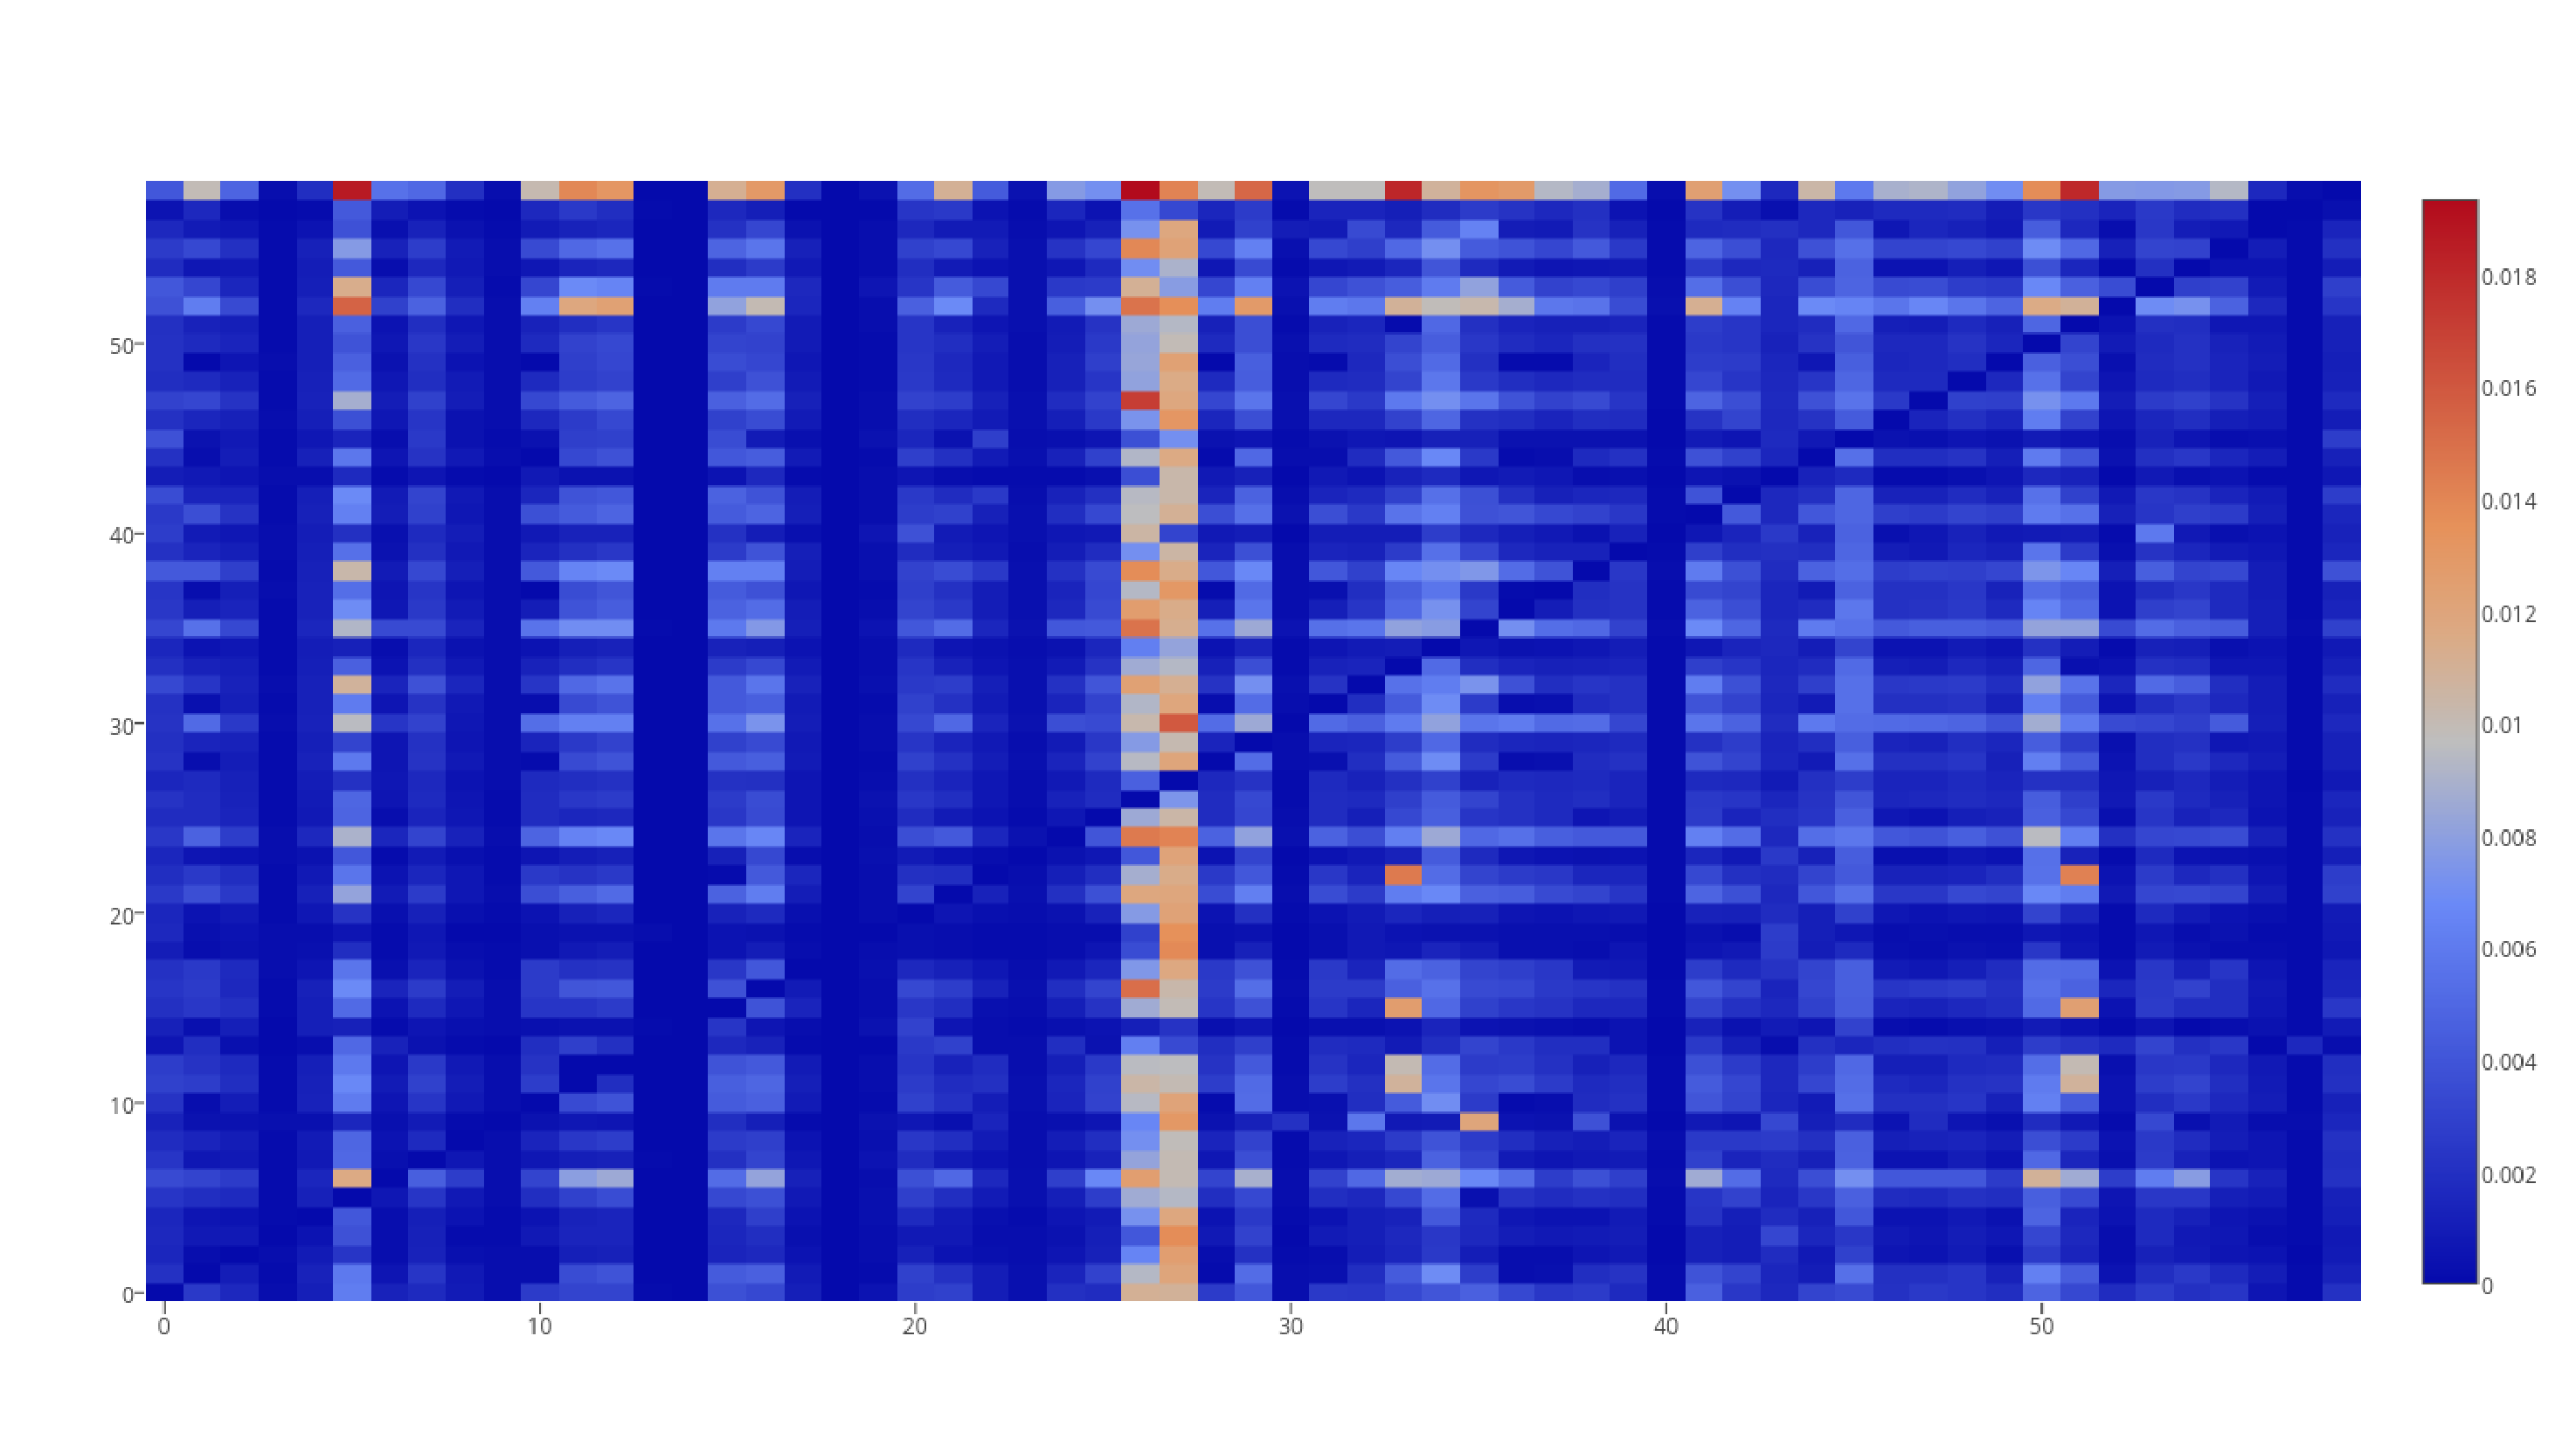
\includegraphics[width=0.24\linewidth]{figure/PC-train}\label{fig:moredata3}} 
\subfloat[]{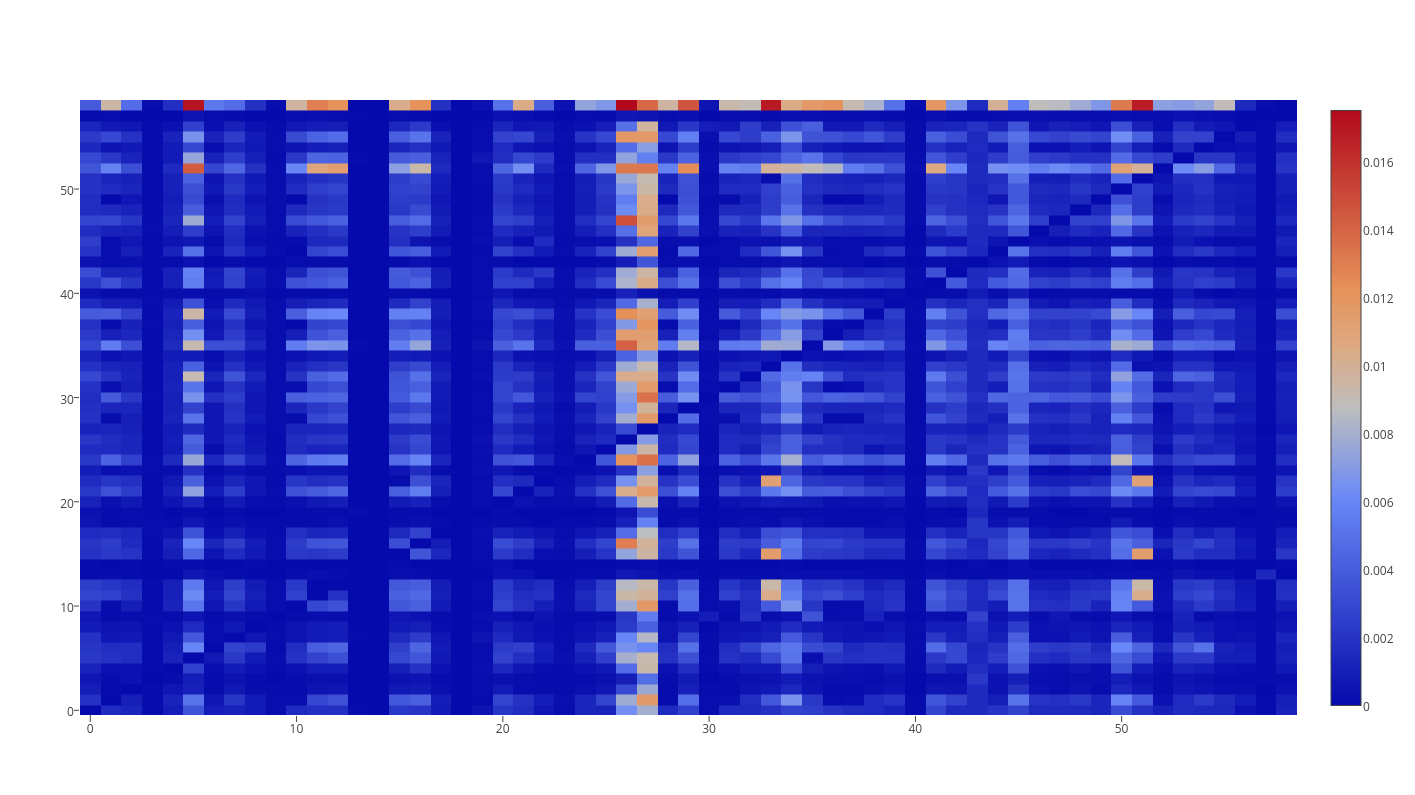
\includegraphics[width=0.24\linewidth]{figure/jaccardPC-train}\label{fig:moredata4}} \\ 
\caption{Potential for 0.5 V bias.} 
\label{fig:EcUND} 
\end{figure*} 


\begin{figure}[t!]
\begin{center}
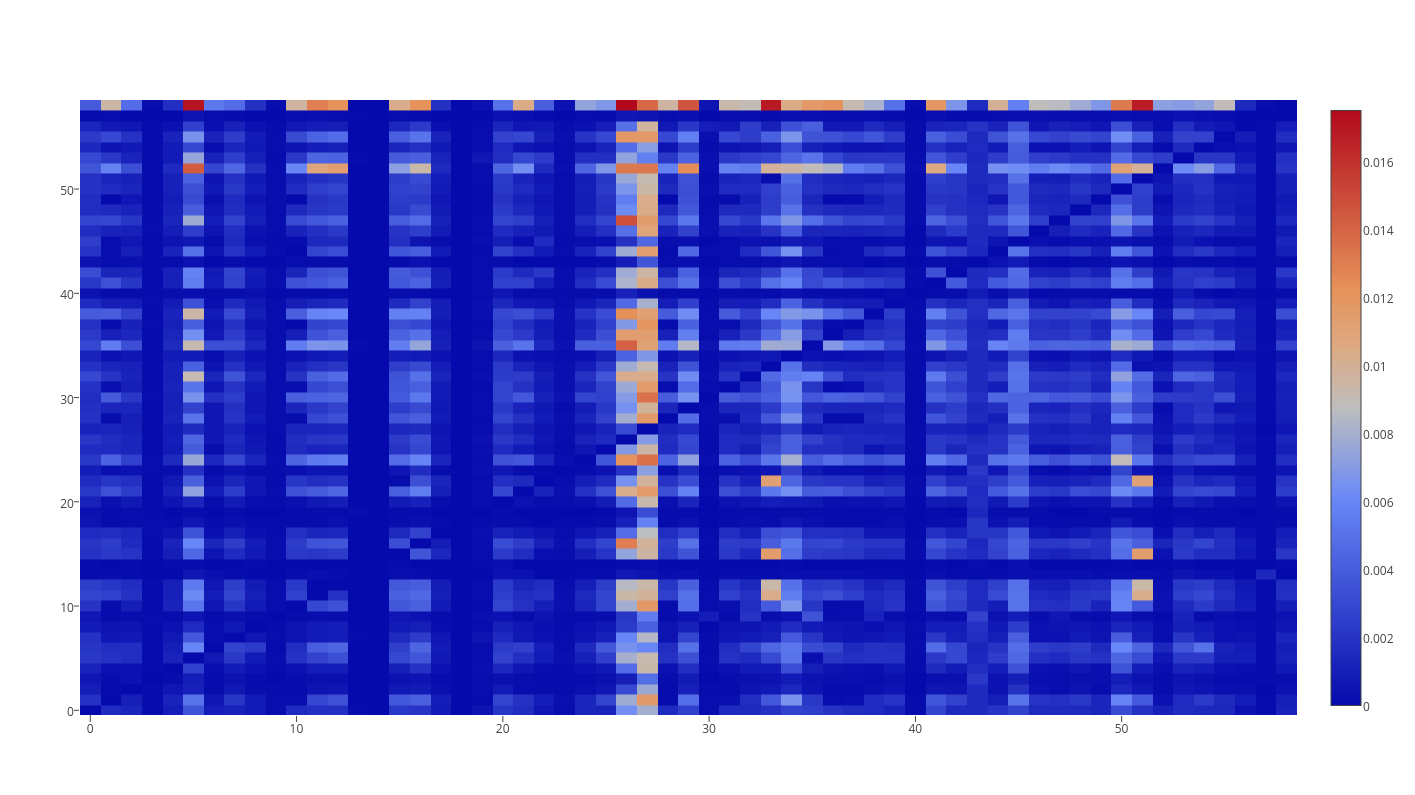
\includegraphics[width=2.5in]{figure/jaccardPC-train}
\mycaption{fig:idreputation}{Test.}
{\footnotesize{(How detection rate changes with the value of source id's reputation. Each reputation is rounded up to nearest 0.05.
Reputation -1 means the source id did not make any submission before. 95\% confidence interval is also drawn 
for each point.)}}
\end{center}
%\vspace{-0.25in}
\end{figure}